\section{Grammar as network of finite automata}

Let's $G$ be an EBNF in which each nonterminal has one rule $A \rightarrow \alpha$, where $\alpha$ is a regular expression over terminals and nonterminals.
The regular expression $\alpha$ defines a regular language and, consequently, there is a finite state automaton $M_A$ that recognizes $\alpha$.

A transition of the grammar $M_A$ labeled with nonterminal $B$ is interpreted as a call to the automaton $M_B$. 
If $B=A$ we the call is termed recursive. 

\begin{definition}
    The finite state automata of the nonterminals of $G$ are called $machines$. 

    The pushdown machine that analyzes $L(G)$ is called $automaton$. 

    The set of all the machines of $G$ is called $network$.
\end{definition}
The elements used to define a network are: 
\begin{enumerate}
    \item The alphabet of the terminal symbols: $\Sigma$
    \item The alphabet of the nonterminal symbols: $V=\{S,A,B,\dots\}$.
    \item The grammar rules: $S \rightarrow \sigma$, $A \rightarrow \alpha$, $B \rightarrow \beta$, etc. 
    \item The regular languages over $\Sigma \cup V$ defined by $\sigma, \alpha, \beta$, etc.: $R_S,R_A,R_B$, etc. 
    \item The deterministic finite machine recognizing $R_S,R_A,R_B$, etc.: $M_S,M_A,M_B$, etc. 
    \item The machine network: $\mathcal{M}=\{M_S,M_A,M_B,\dots\}$
\end{enumerate}

We need to consider also the terminal language defined by a generic machine $M_A$, when starting from a state possibly other than the initial one. 
For any state $q_A$,not necessarily initial, we write as: 
\[L(M_A,q_A)=\{y \in \Sigma^{*}|\exists\eta\in R(M_A,q) \land \overset{*}{\underset{G}{\implies}} y\}\]
The formula above contains a string $\eta$ over terminals and non-terminals, accepted by machine $M_A$ when starting in the state $q$. 
The derivations originating from $\eta$ produce all the terminal strings of language $L(q)$. 
In particular, it follows that: 
\[L(M_A,0_A)=L(0_A) = L_A(G)\]
and for the axiom it is:
\[L(M_S,0_S)=L(0_S)=L_S(G) = L(\mathcal{M})\]

We have to set an additional constraint, that is: the initial state $0_A$ of machine $A$ is never re-entered after the start of the computation. 
This constraint is easily fulfilled, at worst the machine needs a new initial state. 
We say that the automata that satisfy such a condition are normalized. 
\begin{example}
    Consider the grammar for arithmetic expressions: 
    \[
    \begin{cases}
        E \rightarrow [+|-]T((+|-)T)^{*} \\
        T \rightarrow F((\times|/)F)^{*} \\
        F \rightarrow a | '('E')'
    \end{cases}
    \]
    The corresponding network is as follows: 
    \begin{figure}[H]
        \centering
        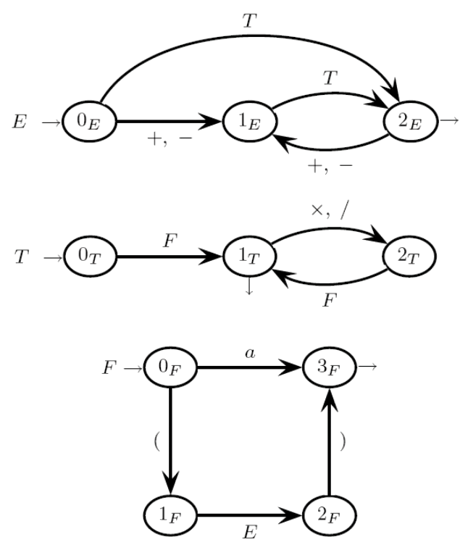
\includegraphics[width=0.4\linewidth]{images/net.png}
    \end{figure}
    Note that the machine $T$ has been normalized. 
\end{example}

These networks can be translated into programs that uses recursion. 
The code of the program reflects the machine transitions. 
When the finite automaton has a bifurcation state, to decide which direction to take we must watch all the symbols that appear on the arcs that leave the state, included the final darts of the machine.
\begin{example}
    The machine net from the previous example can be transformed into three code procedures. 
    The procedure for the grammar $E$ is: 
    \begin{algorithmic}[1]
        \State call $T$
        \While {$cc=+$}
            \State $cc:=next$
            \State call $T$
        \EndWhile
        \If {$cc \in \{(\dashv\}$}
            \State \Return
        \Else 
            \State error
        \EndIf
    \end{algorithmic}
    The procedure for the grammar $T$ is: 
    \begin{algorithmic}[1]
        \State call $F$
        \While {$cc=\times$}
            \State $cc:=next$
            \State call $F$
        \EndWhile
        \If {$cc \in \{(+\dashv\}$}
            \State \Return
        \Else 
            \State error
        \EndIf
    \end{algorithmic}
    The procedure for the grammar $F$ is: 
    \begin{algorithmic}[1]
        \If {$cc=a$}
            \State $cc:=next$
        \ElsIf {$cc=($}
            \State $cc:=next$
            \State call $E$
            \If {$cc=)$}
                \State $cc:=next$
                \If {$cc \in \{) \times \dashv\}$}
                    \State \Return
                \Else 
                    \State error
                \EndIf
            \Else 
                \State error
            \EndIf
        \Else 
            \State error
        \EndIf
    \end{algorithmic}
\end{example}